\section{Local Binary Pattern}

Local binary patterns (LBP) is a type of feature used for classification in computer vision. LBP is the particular case of the Texture Spectrum model proposed in 1990.[1][2] LBP was first described in 1994.[3][4] It has since been found to be a powerful feature for texture classification; it has further been determined that when LBP is combined with the Histogram of oriented gradients (HOG) classifier, it improves the detection performance considerably on some datasets.[5]

Local Binary Pattern (LBP) is a simple yet very efficient texture operator which labels the pixels of an image by thresholding the neighborhood of each pixel and considers the result as a binary number. Due to its discriminative power and computational simplicity, LBP texture operator has become a popular approach in various applications. It can be seen as a unifying approach to the traditionally divergent statistical and structural models of texture analysis. Perhaps the most important property of the LBP operator in real-world applications is its robustness to monotonic gray-scale changes caused, for example, by illumination variations. Another important property is its computational simplicity, which makes it possible to analyze images in challenging real-time settings. 


----

The basic idea for developing the LBP operator was that two-dimensional surface textures can be described by two complementary measures: local spatial patterns and gray scale contrast. The original LBP operator (Ojala et al. 1996) forms labels for the image pixels by thresholding the 3 x 3 neighborhood of each pixel with the center value and considering the result as a binary number. The histogram of these 28 = 256 different labels can then be used as a texture descriptor. This operator used jointly with a simple local contrast measure provided very good performance in unsupervised texture segmentation (Ojala and Pietikäinen 1999). After this, many related approaches have been developed for texture and color texture segmentation.

The LBP operator was extended to use neighborhoods of different sizes (Ojala et al. 2002). Using a circular neighborhood and bilinearly interpolating values at non-integer pixel coordinates allow any radius and number of pixels in the neighborhood. The gray scale variance of the local neighborhood can be used as the complementary contrast measure. In the following, the notation (P,R) will be used for pixel neighborhoods which means P sampling points on a circle of radius of R. See Fig. 2 for an example of LBP computation. 


 An illustration of the basic LBP operator is shown in Figure 3.2
and the corresponding equation is shown below.

R raggio
P pixel in the neighborhood
\begin{equation}
LBP_{P,R}(x, y) = \sum_{p=0}^{P-1}{s(g_p - g_c)2^P}
\end{equation}

\begin{equation}
s(x) = 	\begin{cases} 1, & \mbox{se } x \ge 0 \\ 0, & \mbox{se } x < 0 \end{cases}
\end{equation}

\begin{figure}[ht]
\begin{center}
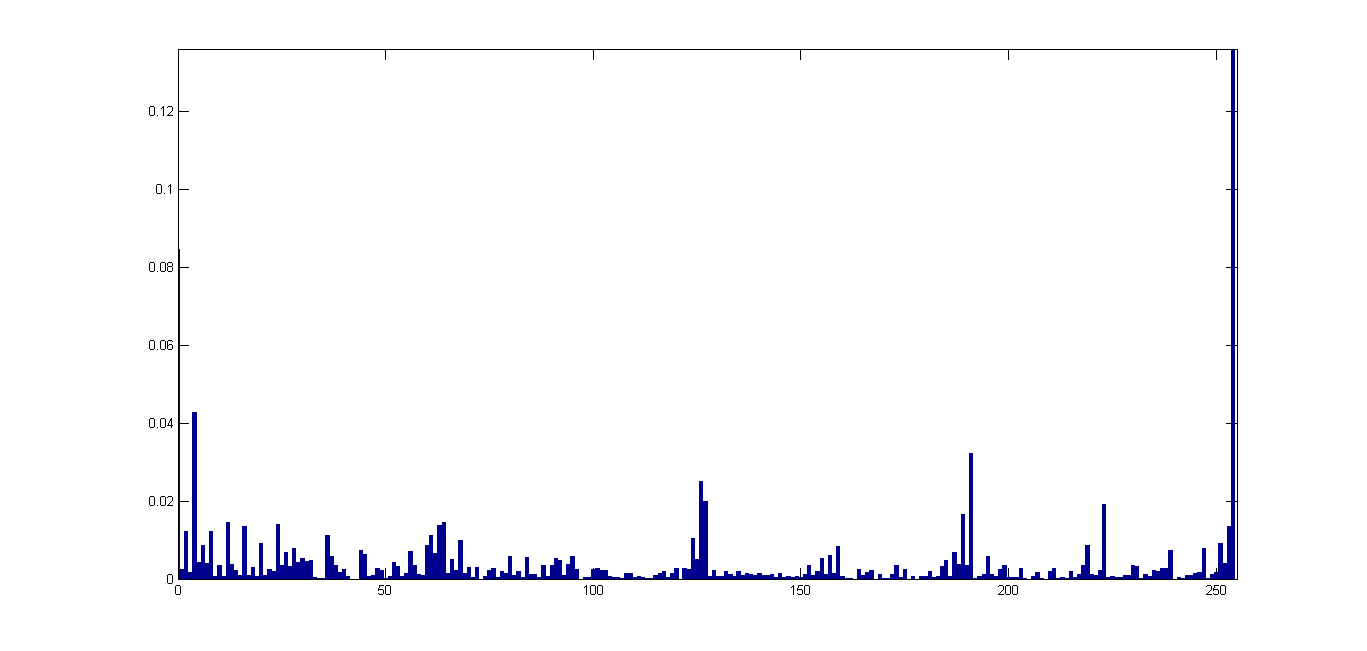
\includegraphics[width=.95\textwidth]{img/hist-complete}
\caption{ Istogramma immagine LBP Base }
\label{fig:istCompleteLBP}
\end{center}
\end{figure}

\begin{figure}[ht]
\begin{center}
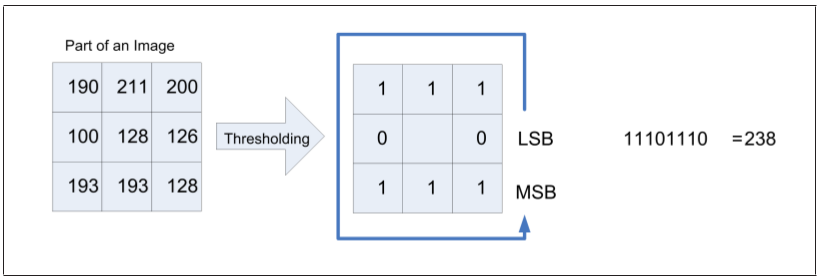
\includegraphics[width=.95\textwidth]{img/LBP_code}
\caption{ Codice LBP }
\label{fig:LBPcode}
\end{center}
\end{figure}



\subsection{Uniform Local Binary Pattern}


Another extension to the original operator is the definition of so called uniform patterns, which can be used to reduce the length of the feature vector and implement a simple rotation-invariant descriptor. This extension was inspired by the fact that some binary patterns occur more commonly in texture images than others. A local binary pattern is called uniform if the binary pattern contains at most two bitwise transitions from 0 to 1 or vice versa when the bit pattern is traversed circularly. For example, the patterns 00000000 (0 transitions), 01110000 (2 transitions) and 11001111 (2 transitions) are uniform whereas the patterns 11001001 (4 transitions) and 01010010 (6 transitions) are not. In the computation of the LBP labels, uniform patterns are used so that there is a separate label for each uniform pattern and all the non-uniform patterns are labeled with a single label. For example, when using (8,R) neighborhood, there are a total of 256 patterns, 58 of which are uniform, which yields in 59 different labels.

Ojala et al. (2002) noticed in their experiments with texture images that uniform patterns account for a little less than 90\% of all patterns when using the (8,1) neighborhood and for around 70\% in the (16,2) neighborhood. Each bin (LBP code) can be regarded as a micro-texton. Local primitives which are codified by these bins include different types of curved edges, spots, flat areas etc. 

\begin{equation}
LBP_{P,R}^{u2}(x, y)	
\begin{cases} 
I(LBP_{P,R}(x, y)), & \mbox{se } U(LBP_{P,R} \le 2, I(z) \in [0, (P-1)P+2 )   \\
(P-1)P+2, & \mbox{altrimenti}
\end{cases}
\end{equation}

\begin{equation}
U(LBP_{P,R} = |s( g_{P-1} - g_{c}) - s(g_{0} - g_{c}) | + \sum_{p = 1}^{P} |s(g_{p} - g_{c}) - s( g_{P-1} - g_{c}) |
\end{equation}


\begin{figure}[ht]
\begin{center}
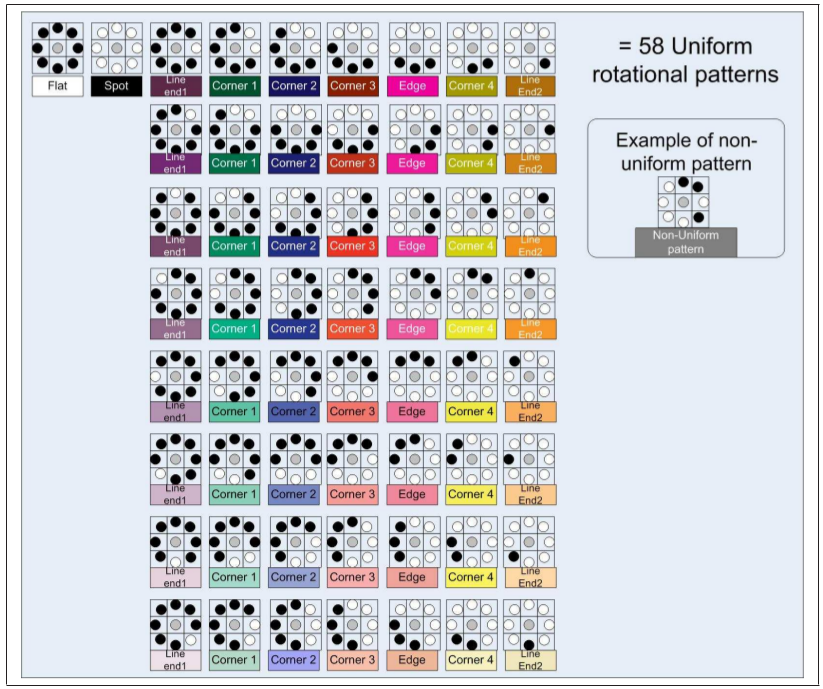
\includegraphics[width=.95\textwidth]{img/uniform_LBP}
\caption{ Uniform LBP }
\label{fig:uniformLBP}
\end{center}
\end{figure}

\subsubsection{Descrittore}

\begin{equation}
h(i) = \sum_{x,y} B(LBP_{P,R}(x, y)) = i, i \in  [0, 2^P-1 ]
\end{equation}

\begin{equation}
B(v) = 	\begin{cases} 1, & \mbox{v = true} \\ 0, & \mbox{altrimenti} \end{cases}
\end{equation}

\begin{figure}[ht]
\begin{center}
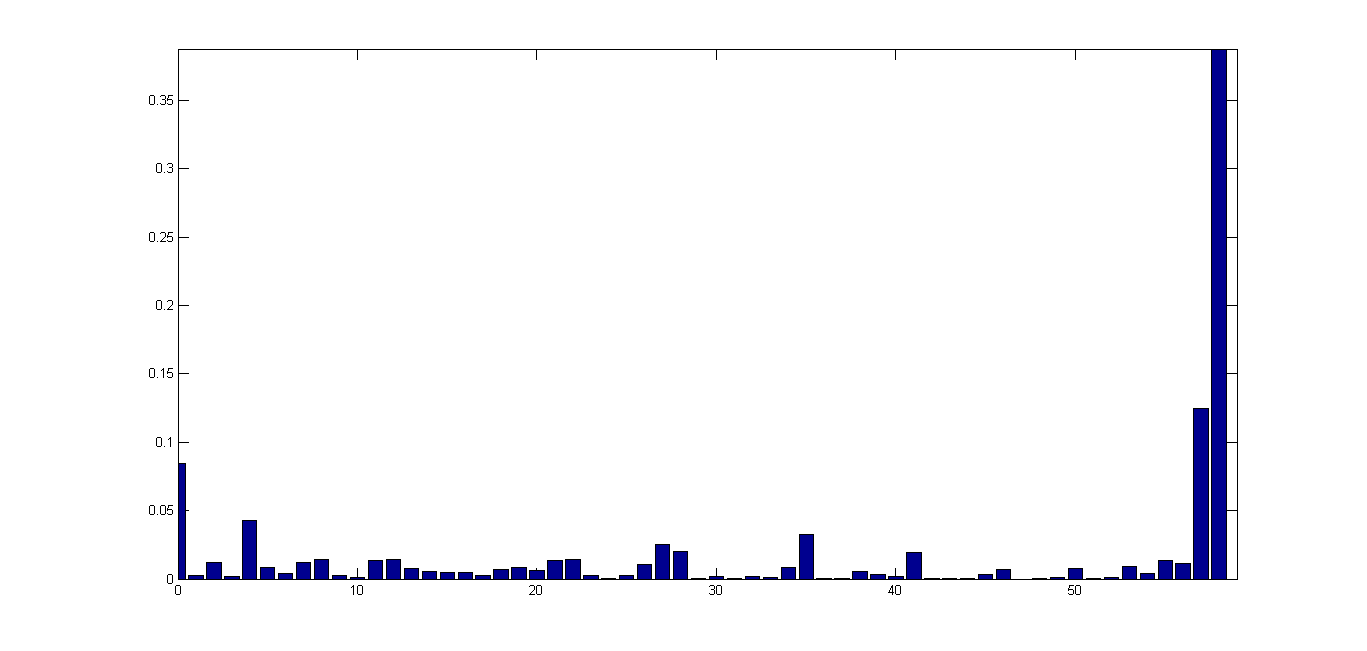
\includegraphics[width=.95\textwidth]{img/hist-uniform}
\caption{ Istogramma immagine LBP Base }
\label{fig:istUniformLBP}
\end{center}
\end{figure}



\subsection{Multiscale Local Binary Pattern}





\begin{figure}[ht]
\begin{center}
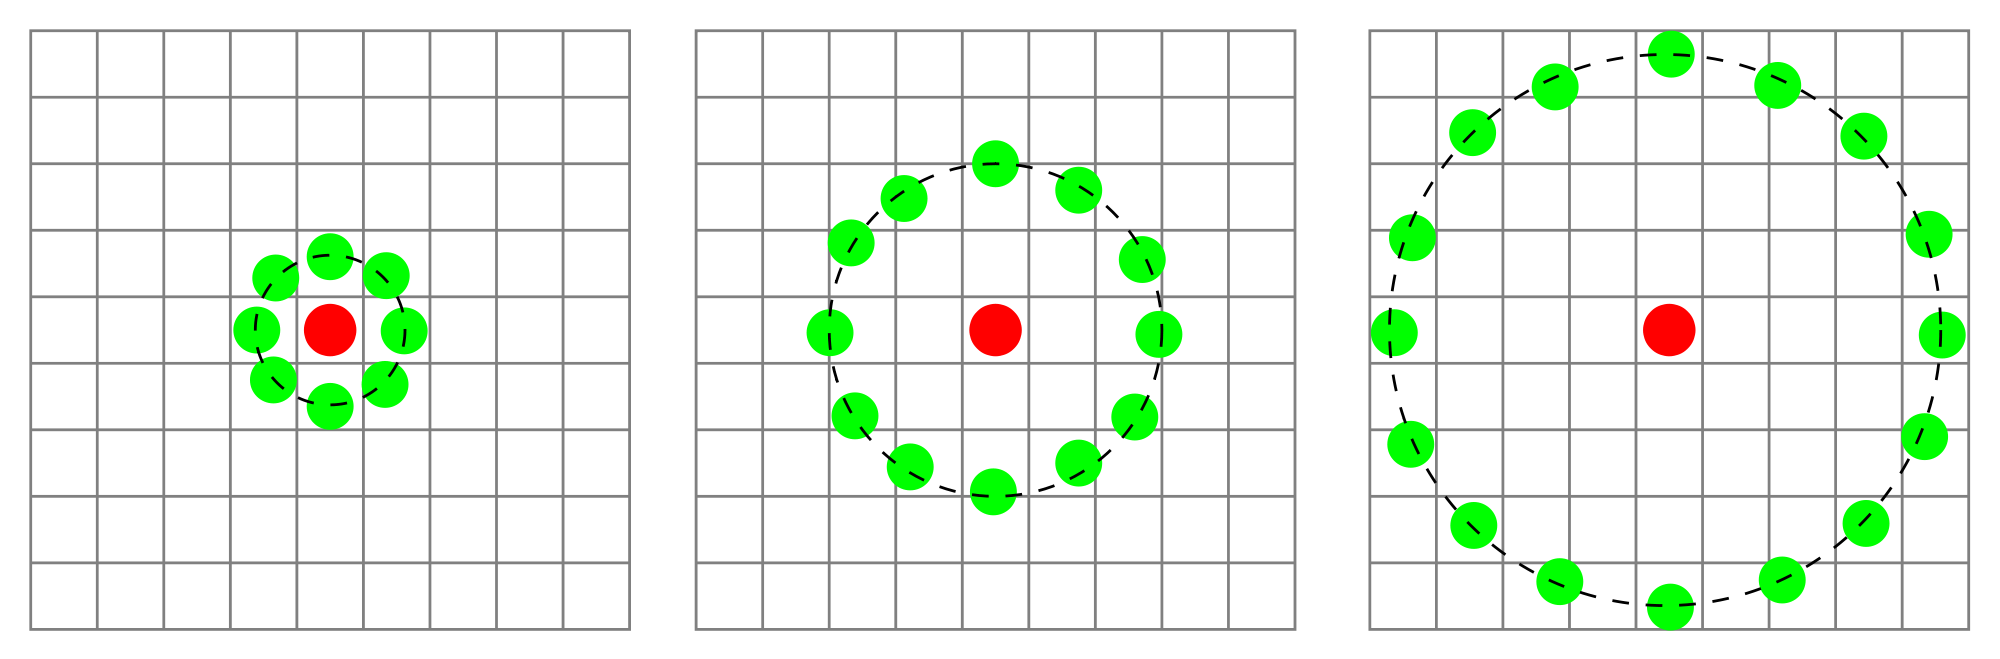
\includegraphics[width=.95\textwidth]{img/raggio_LBP}
\caption{ Multiscale LBP }
\label{fig:MLBP}
\end{center}
\end{figure}

\subsubsection{Descrittore}

j = regione
r = raggio
P = num neighbor
\begin{equation}
h_{P,r,j}(i) = \sum_{x',y' \in M_j} B(LBP_{P,r}(x', y')) = i, i \in  [0, L-1 ], r \in [1, R], j \in [0, J-1]
\end{equation}

\begin{equation}
B(v) = 	\begin{cases} 1, & \mbox{v = true} \\ 0, & \mbox{altrimenti} \end{cases}
\end{equation}

\begin{equation}
f_{j} = [h_{P, 1, j}, h_{P, 2, j}, \cdots, h_{P, R, j}]
\end{equation}

\subsection{Smoothing}